\documentclass{article}
\usepackage[utf8]{inputenc}

\title{Use of asynchronous circuits and leakiness in modeling biological circuit of the Caulobacter Crescentus cell cycle}
\author{Zoey Zhou}
\date{\today}  
\usepackage{graphicx}
\graphicspath{ {c:/Users/cuizy/Downloads/} }
\begin{document}

\maketitle

\section{Intro}
Biological modeling uses from stochastic to continuous to boolean models.  We propose an asynchronous circuit scheme for modeling the cell cycle of the bacteria Caulobacter Crescentus.   Asynchronous circuits are a type of digital circuits where the values are boolean, either 0 or 1, and the boolean functions are implemented through logic gates.  Digital circuits can be synchronous, where all of the logic gates in the circuit are controlled by some global clock, which ensures that the next values for all of the gates are updated at the same time.  Thus problems where various gate delays causing fluctuations in the circuit can be avoided.  In an asynchronous circuit, there is no global clock, and the gates update real time so different computational delay times for each gate cause real effects which may be propagated through the circuit.  Thus for an asynchronous circuit to provide reliable function, these random delays must be designed into the system.  A more stringent condition of asynchronous circuits known as speed independence ensures that no matter the delay for each gate, the circuit will function the same way. 
% different levels of detail

\section{Correct boolean model}
We expect biological systems to behave similarly to an asynchronous circuit because in biological systems there are no 'global clocks' that regulate the timing.  Because there is high variability between cells, and molecular interactions are of a stochastic nature, production from each gene element can have varying delay.  This variability differs from cell to cell and from one cycle to the next. Thus we would also expect a type of speed independence property to ensure that most of the time, the cells work reliably regardless of the random delays and advance through the cell cycle to produce new cells.
\newline \newline
From the bottom up, we extract properties from biological networks and show how it is analogous to the well developed CMOS technology.  We start at the physics level and demonstrate certain properties so that we can group gene elements together and represent them with a higher level boolean model.  We then show how this boolean model can be abstracted into a higher level forming building blocks that we can use in an asynchronous circuit. 
\newline \newline
In past papers, gene regulatory networks has been modeled as boolean circuits with each gene/protein element represented by a boolean gate.  Each gene logic gate has inputs, usually its activators and repressors, to determine whether the protein is being actively produced or not.  These are usually modeled as AND or OR gates with its promoter binding compounds as its only inputs.  However, in our investigation using the ODE model of each gene, we found that degradation is a crucial part of the logic gates as well.  Protein degradation can be sped up through controlling the production of degradation enzymes.  Meanwhile for stable proteins, it is possible for the base degradation rate, the half life of the protein to be equivalent to the length of the cell cycle, the only reduction in protein concentration coming from the splitting of cells.  Thus there needs to be a separate way of representing the production of proteins from its degradation.  We take inspiration from Complementary Metal–Oxide–Semiconductor (CMOS) technology.  In CMOS there is a pull up network and a pull down network.  In the inverter example, the pull up network consists of a PMOS and the pull down network consists of a NMOS.  PMOS behaves, on first order approximation, as a wire when the input voltage is low and as an open circuit when the input voltage is high.  NMOS is the opposite, it behaves as an open when the input voltage is low and as a wire when the input voltage is high.  Thus when the input voltage is low, the output voltage is pulled up by the PMOS to a high voltage.  Meanwhile when the input voltage is high, the output voltage is pulled down to ground by the NMOS.  The transcriptional and translational regulation of these genes are similar to a pull up network while the accelerated degradation is similar to a pull down network.  If the background degradation is significantly slower, this effect can be thought of as the parasitic capacitance that slowly leak the charge of the output signal.  Overtime it degrades the signal however for short time scales it retains its voltage value and is a dynamic memory element.
\newline
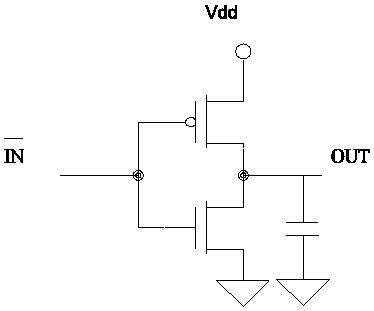
\includegraphics[width=\textwidth]{mosinv}
\newline \newline
Many biological functions can be modeled with the Hill function, including mRNA production.  The sigmoidal shape of the Hill function is reminiscent of Voltage Transfer Characteristics of CMOS inverters.  As such, much of the design properties of CMOS circuits can be carried over.  The importance of the sigmoidal shape of the input vs output transfer curve during steady state allows for restoring property of the signal and hence unsullied propagation in its next stages.   In an ODE model of the protein production and degradation with the Hill function, the steady state solutions are the Hill function divided by the degradation constant.  In general the equation is of the form: $\frac{dprotein}{dt}=g(inputs)-protein\cdot\lambda$  where the function $g()$ is a sigmoidal curve such as the Hill function and $\lambda$ is the degradation constant.  This sigmoidal curve is then an input (the proteins that initiate transcription and production of the protein) versus the output, the current concentration of the protein.  If we treat each protein as its own gate, there exists similar restorative properties of the CMOS gate.
%new, about the thresholds
\newline \newline
The inputs and outputs of electronic devices are similar to the chemical concentrations in a cell which are all actually continuous values (analog).  The concept of a binary '1' or '0' is extracted from the original analog signal.  Thresholds allow the conversion of an analog signal into a binary signal.  Usually there is a low and a high threshold, and an in between region.(figure)  If the signal is below the low threshold then it is a binary '0' and if the signal is above the high threshold it is a binary '1'.  The in between region is undetermined meaning it is neither a '1' or a '0'.   
\newline
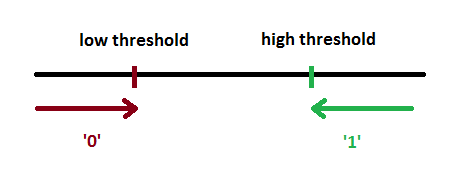
\includegraphics[width=\textwidth]{thresholds}
\newline
One basic property thresolds must satisfy is to allow proper propagation of the signal.  The output of a gate should read as the same binary value into the input of the following gate.  That is for the $i^{th}$ component which is connected to the $i+1^{th}$ component, $output_i low \leq input_{i+1} low$ and $output_i high \geq input_{i+1} high$.  There is a naturally defined output threshold given the input thresholds.  That is passing the input threshold through the gate function G(). In addition, if the signal is monotonic then all inputs below the input low threshold or above the input high threshold gives valid output signals as well.  The reasoning is because for all $input low$ $x_i$ pairs, where $input low>x_i$ then $G(input low)>G(x_j)$ since G() is monotonic.  We also need to consider multiple input systems such as in biology where there can be multiple inputs to the same gate.  In biological systems where the ODE model is a sigmoidal curve in the form of a Hill function, the partial derivative with respect to any one input variable is always monotonic.  Thus this satisfies our monotonic requirement and allow for proper propagation.  In addition, because these equations are monotonic with regard to any one variable, there are only a limited number of logic that can be formed.  (expand?)
\newline
The other property that sigmoidal curves are important for is the restorative property of signals to allow for noise and increase robustness.  
%Sigmoidal, All the things about how they connect, why they are good latches/ memory elements, completion signals?
\section{Static and Dynamic Memory}
There are certain network motifs that we have identified in our model of Caulobacter that allows cells to have some sort of memory.  There are positive feedback loops such as in CtrA where once enough production of CtrA starts the feedback, it will remain locked in that high state.  Until degradation overpowers the feedback and pulls CtrA back down to a low state.  This bistable property is also how latches in digital circuits store memory.  However for other proteins that do not have this positive feedback, we take inspiration from dynamic memory and look into the short term behavior instead.  As mentioned earlier, when the degradation term is slow the actual changes in protein concentration over time is slow as well and can act as a memory element.  If we assume the inputs are held constant, there is a closed form exponential solution to our ODE model.  (z is the output protein concentration)
$\Delta t= -log(z_f-z_{ss})/ \lambda+ log(z_0-z_{ss})/ \lambda$ This is the amount of time it takes for the protein concentration to go from $z_0$ to $z_f$, initial protein concentration to final protein concentration, with a steady state concentration due to the input parameters of $z_{ss}$.
\newline
In a set reset gate, there are two inputs, both of which must be 1 to set the output to 1, and both must be 0 to set the output to 0.  If one input is 0 and one is 1 then the output does not change and is in the hold state.  This is an important element for constructing asynchronous digital circuits.  
In our model we wish to verify the set reset property of each gene gate.  We use the above equation to check if the time for maximum set or reset transitions is smaller than the time during the hold state.  
Let the input thresholds be:  0 is between $in_{min0}$ and $in_{max0}$ and 1 is between $in_{min1}$ and $in_{max1}$, (the fanout thresholds $fanout_0$ and $fanout_1$ must be between $g(in_{max0})$ and $g(in_{min1})$ )
The maximum time it takes to set or reset in terms of output values is then: \newline
Set- $out_{min0}$ - $fanout_1$ where the input is changed to inmin1 \newline
Reset- $out_{max1}$ - $fanout_0$ where the input is changed to inmax0 \newline
For holds we want the minimum time it stays in output 0 or 1 as the inputs are changed \newline
$out_{max0}$ - $fanout_0$ with max \newline
$out_{min1}$ - $fanout_1$ \newline
\[\Delta t_{set}= - \frac{1}{\lambda} log(g(in_{min1})-fanout_1)/(g(in_{min1}) -g(in_{min0}))
\]
\[\Delta t_{reset}= -\frac{1}{\lambda} log(fanout_0 –g(in_{max0}))/(g(in_{max1}) – g(in_{max0}))
\]
\[\Delta t_{hold0}= -\frac{1}{\lambda} log(z_{ss} -fanout_0)/(z_{ss} -g(in_{max0}))				
\]
\[\Delta t_{hold1}= -\frac{1}{\lambda} log(fanout_1 -z_{ss})/(g(in_{min1}) -z_{ss})
\]

\newline Using standard parameter values, it is possible to have the hold times to be longer than the set reset times and so for short periods of time, this element can be considered as a set-reset memory element.  Thus we can abstract these biological motifs as a series of static and dynamic memories connected to each other.


\section{Leakiness}
Interestingly, there are a couple examples even in the Caulobacter cell where if you knockout one of the key components of the core cell cycle proteins that the rest of the cycle still tries to proceed.  For example, experiments where GcrA or CcrM has been deleted should halt the cell cycle since they start the transcription of CtrA and DnaA respectively.  However, it has been shown that after some delay DnaA and CtrA levels accumulate enough such that the cell can enter the next phase of the cycle.  This may be attributed to a base rate of leakiness from their promoters and other stochastic effects.  We analyze the likely causes of this observation.

CtrA has positive self-feedback.  Plotting the solutions of the Hill kinetics and a diagonal line, representing that all CtrA are phosphorylated to CtrAP during this feedback, shows that this causes CtrA to be bistable. (figure \ref{fig:ctrapc})  However if you include leakiness of the promoter, that shifts the curve of CtrAP vs CtrA up such that even in the presence of no CtrAP, there is still some CtrA produced from the base rate.  If the leakiness from the promoter is large enough, it can shift the curve up so much that there is only one stable point of the system, where ctrA is high. (figure \ref{fig:ctrapl}) This would explain why deletion of GcrA and the P1 promoter where GcrA binds to delays the accumulation of CtrA.  In an earlier paper \cite{compgenre} Michaelis-Menton (MM) kinetics was used.  In their model, they also observed a restart of CtrA even when the upstream transcription factor GcrA was not present.  This is because the MM curve produces only one stable equilibrium so CtrA will always go high if given enough time.

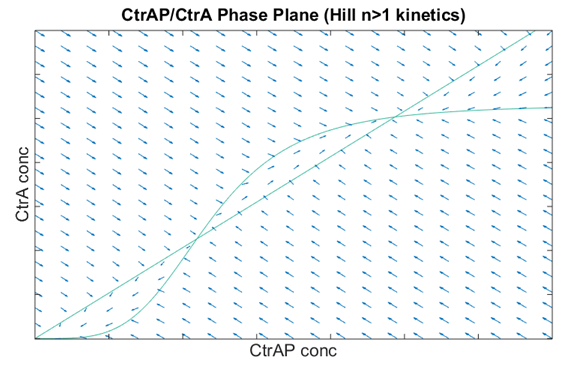
\includegraphics[width=\textwidth]{ctrapc}
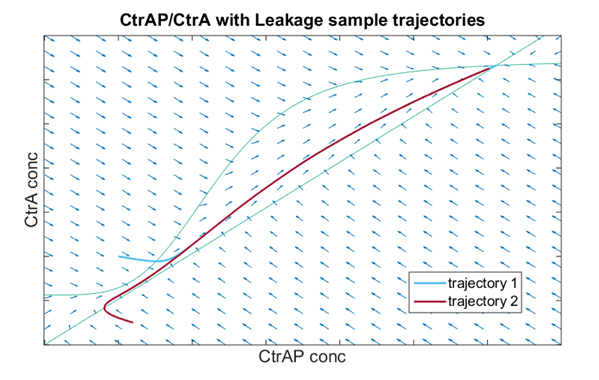
\includegraphics[width=\textwidth]{ctrapl}
\newline \newline
For DnaA, there is evidence that in cells with DnaA lacking the CcrM binding site, the phenotype is not as severe as deleting DnaA directly.  Instead the cell cycle is slowed down.  Thus, there is reason to believe that DnA is also controled by a leaky promoter.  

\begin{thebibliography}{9}
\bibitem{compgenre} 
S M Murray, G Panis, C Fumeaux, P H Viollier , M Howard. 
\textit{Computational and Genetic Reduction of a Cell Cycle to Its Simplest, Primordial Components}. 
PLOS Biology, December 31, 2013.
 
\end{thebibliography}
	
\end{document}
